\chapter{Gradu Amaierako Proiektuaren Formatua}
\label{ch:aurkezpena}


% Goiburukoan agertuko den testua (kapituluko izenaren desberdina izatea mnahi bada)
\chaptermark{GAP}


\section{Formatua}
\label{atala:formatua}


Hemen zure dokumentua idatzi beharko duzu. Atalak \texttt{section} hitzaz \\
(\verb+\section{Sarrera}+) eta azpiatalak \texttt{subsection} (\verb+\subsection{Zerrendak}+) moduan adierazi beharko dituzu.

Sarean \LaTeX{}-ren inguruko eskuliburu anitz dituzu, beraz, ez zenuke arazorik beharko idazteko. Hona hemen batzuk:

\vspace{0.25cm}

\url{http://es.wikibooks.org/wiki/Manual\_de\_LaTeX}

\url{http://en.wikibooks.org/wiki/LaTeX}

\url{http://itsas.ehu.es/workgroups/latex/recetas}

\vspace{0.15 cm}

Dokumentu honetan \LaTeX{} erabiltzeko oinarrizkoak diren ideia batzuk ageri dira. Iturria, \emph{4-examples-eu.tex}, irekitzea gomendatzen dizut, aginduak nolakoak diren ikusteko. Edozein kasutan, dokumentu honetan kodearen zati batzuk ikusi ahal izango dituzu.

Testuan oharrak idatzi nahi badituzu eta hauek ez ikustea nahi baduzu, erabili ``\%'' ikurra aurretik.

% Honela


\subsection{Zerrendak}
\label{azpiatala:zerrendak}

Bi zerrenda mota erabiltzen dira gehien.

Zenbakidunak:
\begin{enumerate}
\item Bat
\item Bi
\item Hiru
\end{enumerate}

Kodea:

\vspace{0.25 cm}

\begin{minipage}{8cm}
\begin{verbatim}
  \begin{enumerate} 
  \item Bat
  \item Bi
  \item Hiru
  \end{enumerate} 
\end{verbatim}
\end{minipage}

\vspace{0.5 cm}

Zenbakirik gabekoak:
\begin{itemize}
\item Atea
\item Bakailua
\item Zuhaitza
\end{itemize}

Kodea:
\vspace{0.5 cm}

\begin{minipage}{8cm}
\begin{verbatim}
  \begin{itemize}
  \item Atea
  \item Bakailua
  \item Zuhaitza
  \end{itemize}
\end{verbatim}
\end{minipage}

\subsection{Taulak}
\label{azpiatala:taulak}

Taulak  \LaTeX{}-en barne"-algoritmo baten bidez kokatzen dira. Beraz, normalean programak kokatuko ditu egokien iruditzen zaion tokian. Hala ere, kokalekua zehatz daiteke idazlearen preferentziak adieraziz.  


\begin{table}[ht]
% hemen aukerak h (here), t (top), b (botton), p (next page)
% Aukeren preferentziak: [htbp]
% Derrigortu hemen ipintzera: [!h] (ez du beti kasu egiten)
\begin{center}
   \begin{tabular}{|l|rl|}
      \hline \bf Irakasgaia & \bf Lauhilekoa & \bf Kredituak \\ \hline
              Oinarrizko Programazioa & 1 & 6 \\
              Analisi Matematikoa & 1  & 6 \\
              Programazioaren Metodologia & 2  & \\
              Kalkulua& 2 pt & 6 \\
       \hline
   \end{tabular}
\end{center}
\caption{\label{Ir-1} II Graduan irakasgai batzuk. }
\end{table}

\vspace{4 cm}

Kodea:

\vspace{0.5 cm}

\begin{minipage}{8cm}
\begin{verbatim}
\begin{table}[ht]
% hemen aukerak h (here), t (top), b (botton), p (next page)
% Aukeren preferentziak: [htbp]
% Derrigortu hemen ipintzera: [!h] (ez du beti kasu egiten)
\begin{center}
  % Marrak non eta l-left, r-right, c-center
  \begin{tabular}{|l|rl|} 
    \hline 
    \bf Irakasgaia & \bf Lauhilekoa & \bf Kredituak \\ 
    \hline
     Oinarrizko Programazioa & 1 pt & 6 \\
     Analisi Matematikoa & 1 pt & 6 \\
     Programazioaren Metodologia & 2 pt & \\
     Kalkulua& 2 pt & 6 \\
       \hline
   \end{tabular}
\end{center}
\caption{\label{Ir-1} II Graduan irakasgai batzuk. }
\end{table}
\end{verbatim}
\end{minipage}

\vspace{0.5 cm}

Kodean ikusten duzun \verb+\label{}+ etiketaren bitartez, taulei, irudiei eta atal eta azpiataleri erreferentzia egin ahalko diezu, zein zenbaki duten ezagutu gabe.

Adibidez, `` \ref{Ir-1} taulan gure fakultateko lehen mailako irakasgaiak ikus ditzakezu''. Erreferentzia egiteko: (\verb+\ref{Ir-1} taulan+).

\vspace{0.5 cm}

\subsection{Irudiak}
\label{azpiatala:irudiak}

Jarraian \ref{fig:infor-sarrera} irudian Informatika Fakultateko sarrera ikus dezakezue.


\begin{figure}[htbp] 
  \begin{center} 
    \scalebox{0.4}{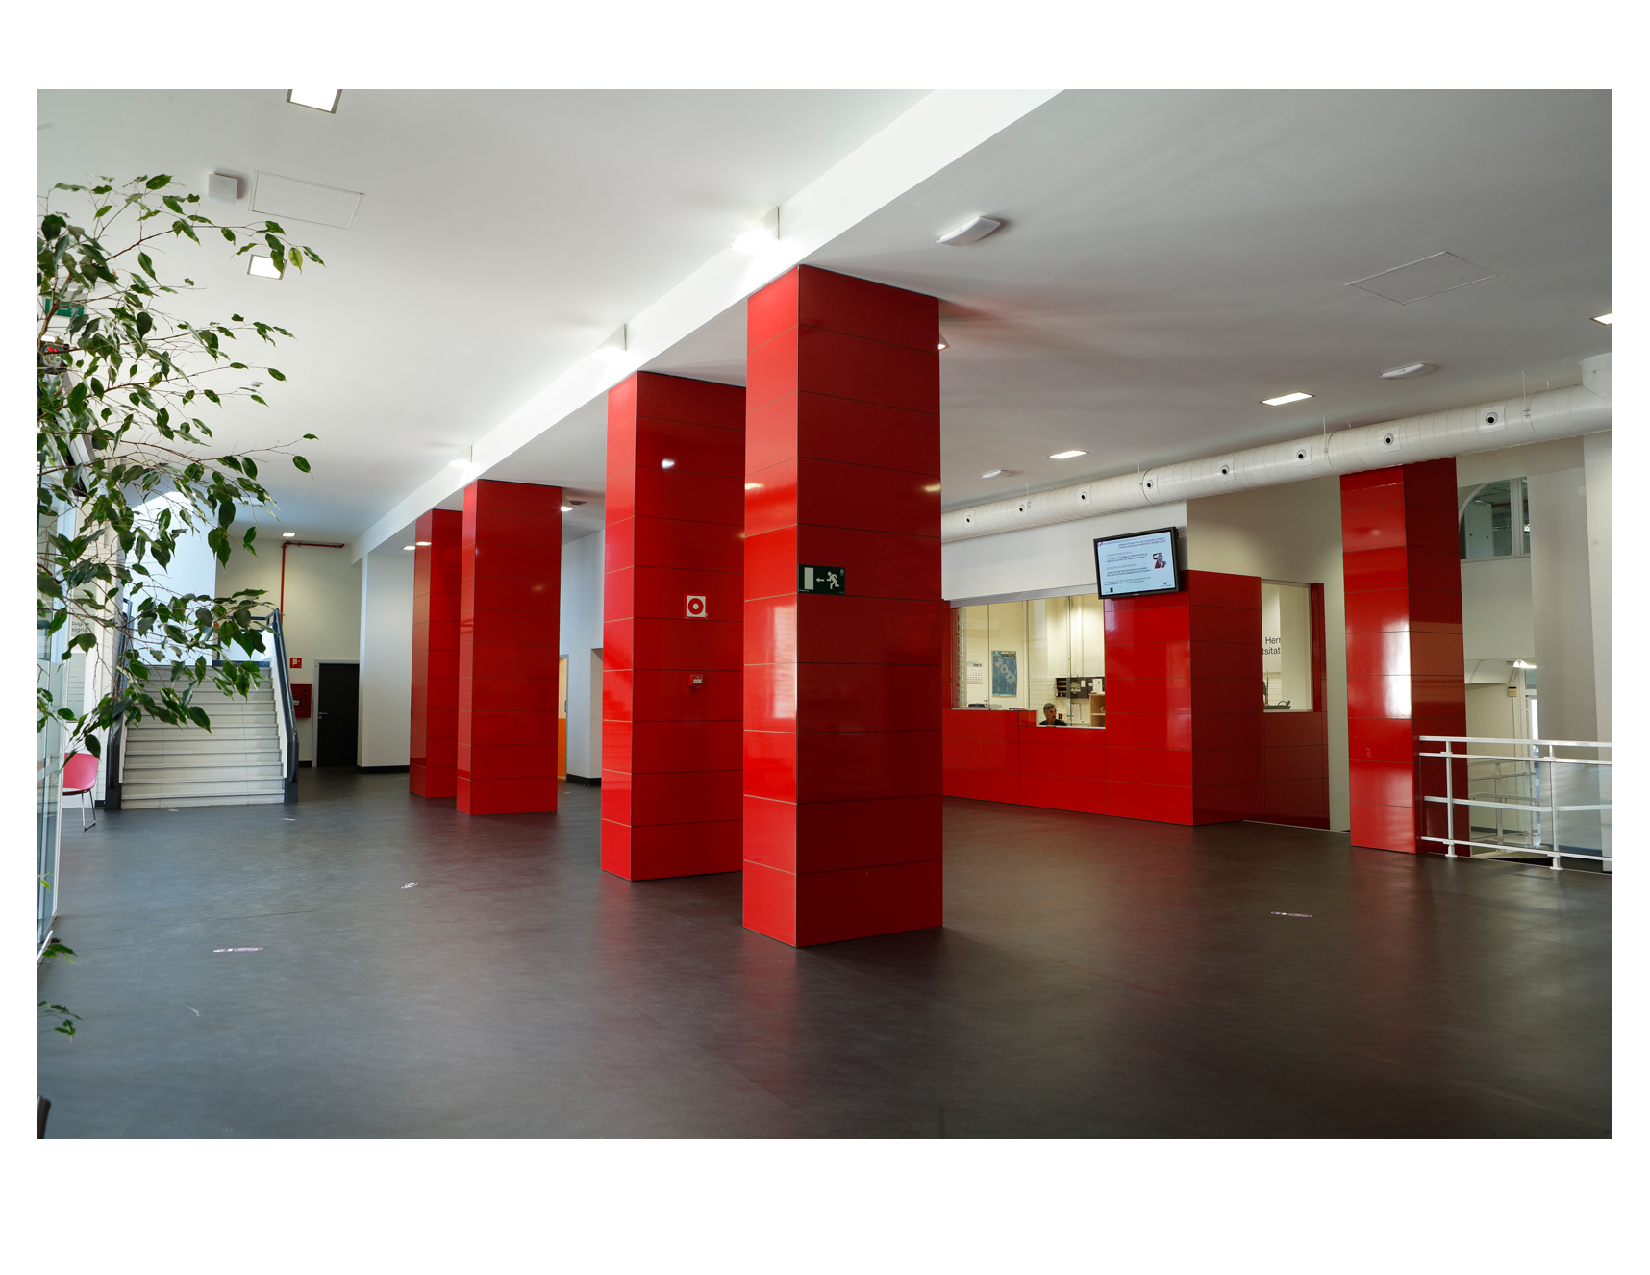
\includegraphics{figs/hall.pdf}} 
    \caption{\emph{Informatika Fakultate}ko sarrera.} 
    \label{fig:infor-sarrera} 
  \end{center} 
\end{figure}

Kodea:
\vspace{0.5 cm}

\begin{minipage}{8cm}
\begin{verbatim}

\begin{figure}[htbp] 
  \begin{center} 
    \scalebox{0.4}{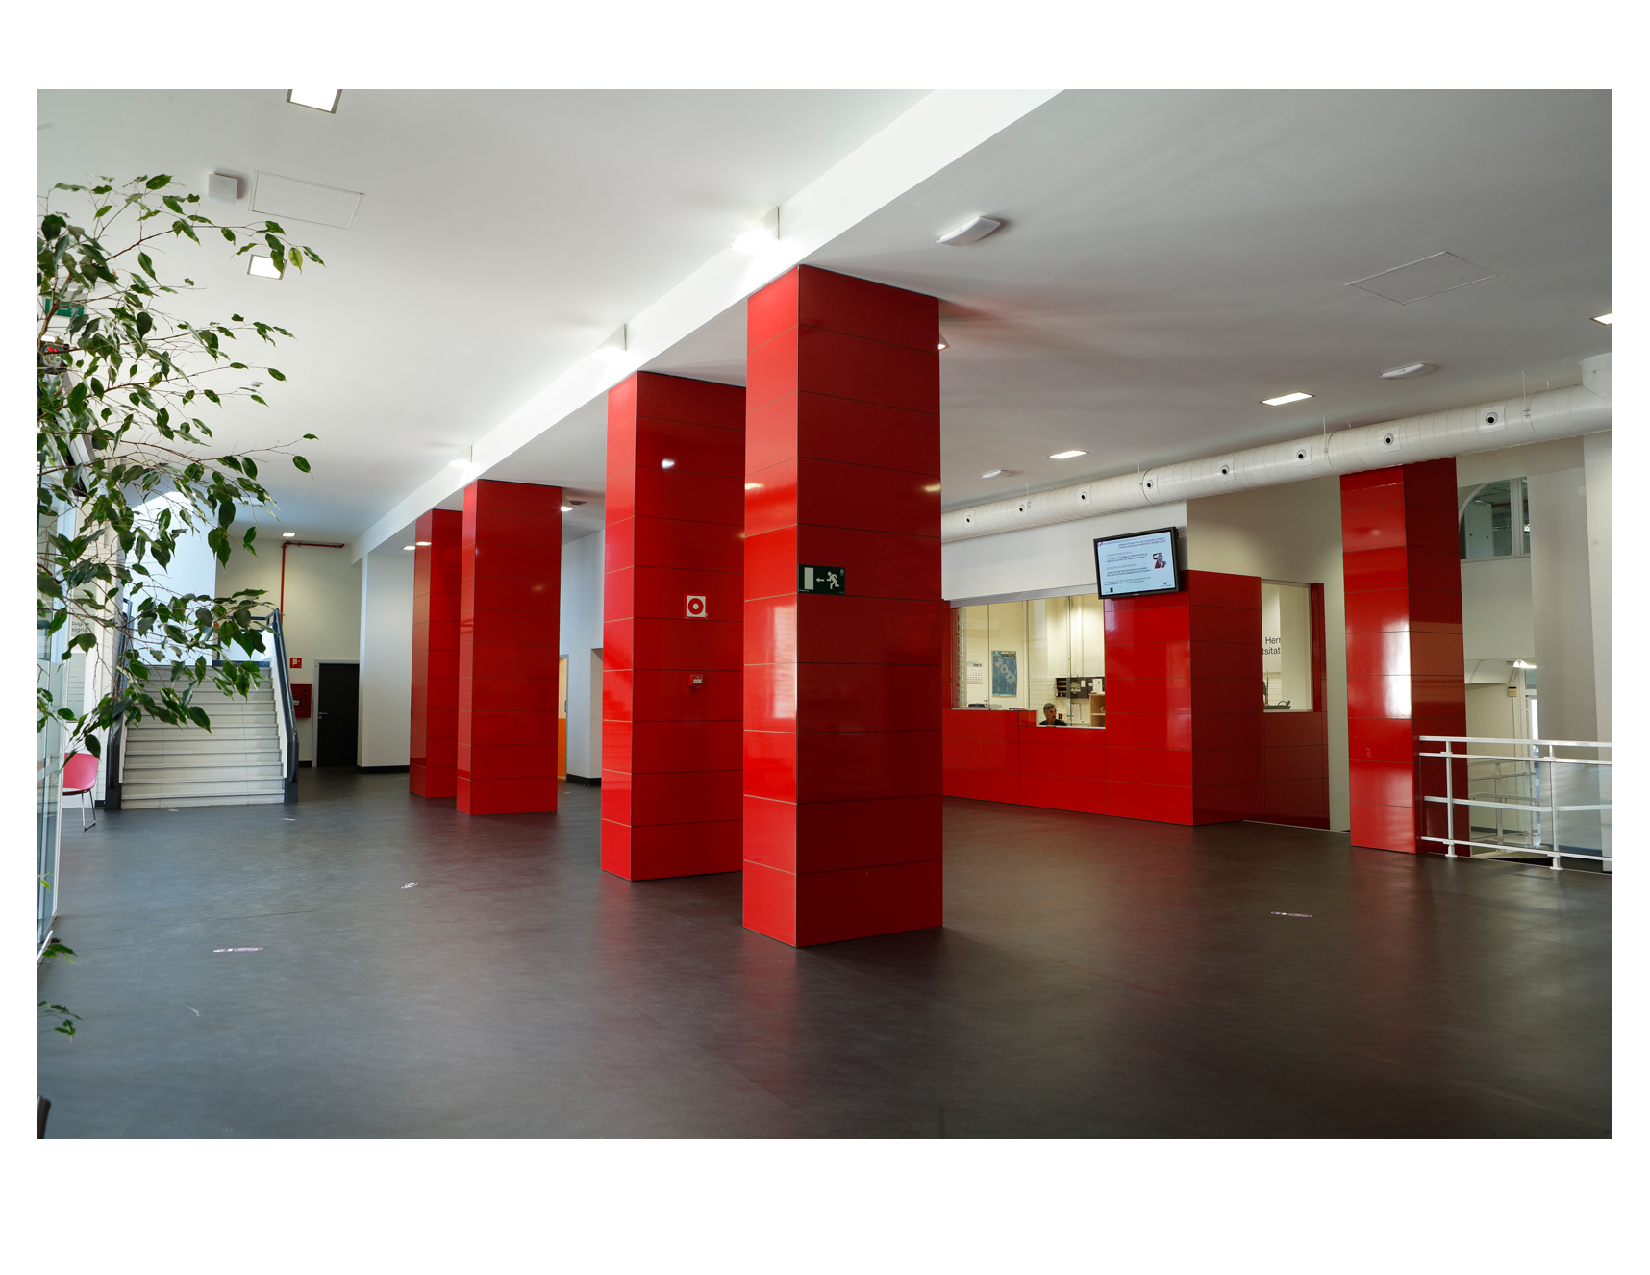
\includegraphics{figs/hall.pdf}} 
    \caption{\emph{Informatika Fakultate}ko sarrera.} 
    \label{fig:infor-sarrera} 
  \end{center} 
\end{figure}

\end{verbatim}
\end{minipage}


\subsection{Letra"-motak}
\label{azpiatala:letra}


Testua bai \textbf{beltzez} (\verb+\textbf{beltzez}+), edo letra \emph{etzanaz} (\verb+\emph{etzanaz}+) edo \textit{italikaz} (\verb+\textit{italika}+) idatz dezakezu. Baita \textsc{hizki"-larri txikietan} (\verb+\textsc{hizki-larri txikietan}+) ere.


Gainera hizkiaren tamaina alda dezakezu:

\begin{itemize}
 \item {\tiny honela}(\verb+{\tiny honela}+)
 \item {\scriptsize honela} (\verb+{\scriptsize honela}+)
 \item {\footnotesize honela} (\verb+{\footnotesize honela}+)
 \item {\small honela} (\verb+{\small honela}+)
 \item {\normalsize honela} (\verb+{\normalsize honela}+)
 \item {\large honela} (\verb+{\large honela}+)
 \item {\Large honela} (\verb+{\Large honela}+)
 \item {\LARGE honela} (\verb+{\LARGE honela}+)
 \item {\huge honela} (\verb+{\huge honela}+)
 \item {\Huge honela} (\verb+{\Huge honela}+)
 \item \ldots 
\end{itemize}


\subsection{Bibliografia}
\label{azpiatala:biblio}

Bibliografia oso modu egokian lantzen da \LaTeX{}"-en. Liburu, artikulu edo web"-orrien erreferentziak aparteko fitxategi batean biltegiratzen dira.

Adibide honetan ``main.tex''-en arabera erreferentziak \emph{bibliografia} izeneko fitxategian (\verb+\bibliography{bibliografia}+), biltegiratuta daude honako moduan:
 
\vspace{0.25 cm}

Kodea:
\vspace{0.25 cm}

\begin{minipage}{8cm}
\begin{verbatim}
@book{DBLP:books/aw/Lamport86,
	author    = {Leslie Lamport},
	title     = {LaTeX: User's Guide {\&} Reference Manual},
	publisher = {Addison-Wesley},
	year      = {1986},
	isbn      = {0-201-15790-X},
	bibsource = {DBLP, http://dblp.uni-trier.de}
}
\end{verbatim}
\end{minipage}

\vspace{0.25 cm}

Gero, testuan aipamena egiteko, adibidez, (\cite{DBLP:books/aw/Lamport86}), zera idatzi behar da: \verb+\citep{DBLP:books/aw/Lamport86}+.

Testuaren barruan erreferentzia egiteko, adibidez, \cite{DBLP:books/aw/Lamport86}-ren arabera honako modua erabili behar duzu:  

\verb+\cite{DBLP:books/aw/Lamport86}+.


\subsection{Footnotes}
\label{azpiatala:oin-oharrak}

Footnote edo oin"-oharrak\footnote{Adibide moduan ohar txiki bat.} \verb+\footnote{}+ aginduaz ipintzen dira.



\section{Erderetako terminoen itzulpena}
\label{azpiatala:erdarak}

Orokorrean, bestelako hizkuntzetatik itzulitako terminoak, ingelesetik adibidez, letra"-etzanez idatziko dira. Adibidez, \emph{on"-line}, \emph{wrapper}, \emph{proxy} \ldots


% Ondorengo lerroak ipinita, fitxategi hontatik bertatik konpilatu ahal izango duzu dokumentua


%%% Local Variables: 
%%% mode: latex
%%% TeX-master: "../NAGUSIA"
%%% End: 





















% line in order to check if utf-8 is properly configured: áéíóúñ
